\section{Architecture}
In our system we have a set of classes which are central to the 
game. Those classes handle theming, player actions, game logic 
and the graphical representation of the game. These central
classes of our game are depicted in Fig.\ref{fig:architecture}.
%
\begin{figure}[tbh]
  \begin{center}
    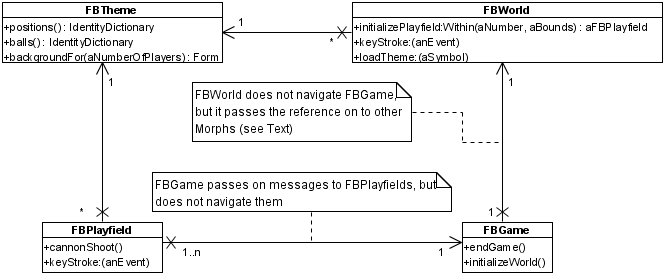
\includegraphics{images/architecture.png}
  \end{center}
  \caption{The central system architecture}
  \label{fig:architecture}
\end{figure}
%
The first instanciated class is FBGame. FBGame controls the game functionality, 
like the number of players, reward strategies like highscores and the
conditions of victory and defeat. FBGame is also responsible for instanciating
the FBWorld class which encapsulates graphical representation of the game.

FBWorld is passed a symbol at startup, which is resolved to a FBTheme. FBWorld 
holds a reference to the current theme and creates its main submorphs, like
a menu, highscore list the changing backgrounds and the in-game playfields.
These Morphs, however, are not held in an instance variable of any kind, but 
are returned to the FBGame instance, for co-ordination.\\
Out of technical necessity, FBWorld also catches all keytrokes, handling them, 
however, is up to the FBGame. Global events, like pause and quit, are handled 
directly, all other keystrokes are passed on to all playfields in the game (if any)
and handled there.

FBPlayfields are created by the world upon the requirements of the theme
and then returned to the FBGame. The playfields receive their own reference 
to the theme and are themselves responsible for their content and reaction on 
player input.

The theme class is implemented as flyweight, holding references to previously 
created instances of a particular theme. If a requested theme type is not yet 
held in the list of instances, the class calls a builder class, 
FBThemeBuilder~\ref{fig:system}, to parse the requested theme's XML file, 
load the images and then return a fresh instance of the theme.
%
\begin{figure}[tbh]
  \begin{center}
    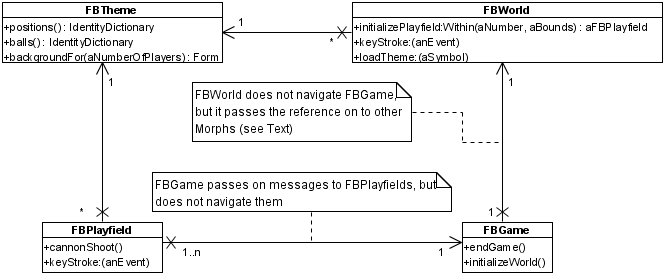
\includegraphics{images/architecture.png}
  \end{center}
  \caption{The complete system overview}
  \label{fig:system}
\end{figure}
%

